% Auto-generated by the analysis pipeline — do not edit
% y > 0: Underreacts  |  y < 0: Overreacts
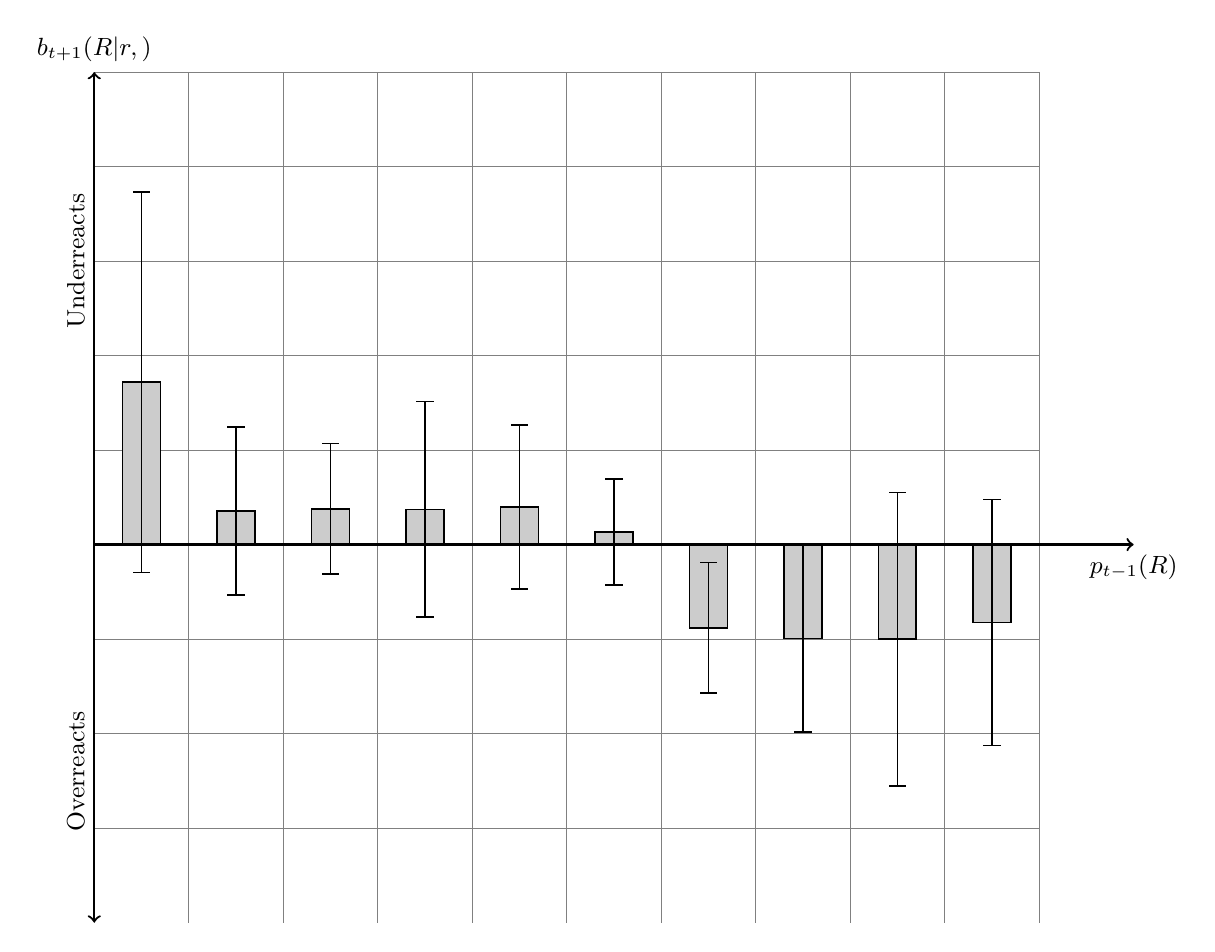
\begin{tikzpicture}[scale=12]
\draw[help lines,step=0.1] (0,-0.4) grid (1,0.5);
\filldraw[opaque,white!80!black] (0.03,0) rectangle (0.07,0.1718);
\draw[line width=0.6] (0.03,0) rectangle (0.07,0.1718);
\draw[line width=0.6,|-|] (0.05,-0.0306) -- (0.05,0.3742);
\filldraw[opaque,white!80!black] (0.13,0) rectangle (0.17,0.0356);
\draw[line width=0.6] (0.13,0) rectangle (0.17,0.0356);
\draw[line width=0.6,|-|] (0.15,-0.0540) -- (0.15,0.1251);
\filldraw[opaque,white!80!black] (0.23,0) rectangle (0.27,0.0378);
\draw[line width=0.6] (0.23,0) rectangle (0.27,0.0378);
\draw[line width=0.6,|-|] (0.25,-0.0323) -- (0.25,0.1079);
\filldraw[opaque,white!80!black] (0.33,0) rectangle (0.37,0.0373);
\draw[line width=0.6] (0.33,0) rectangle (0.37,0.0373);
\draw[line width=0.6,|-|] (0.35,-0.0777) -- (0.35,0.1523);
\filldraw[opaque,white!80!black] (0.43,0) rectangle (0.47,0.0395);
\draw[line width=0.6] (0.43,0) rectangle (0.47,0.0395);
\draw[line width=0.6,|-|] (0.45,-0.0482) -- (0.45,0.1272);
\filldraw[opaque,white!80!black] (0.53,0) rectangle (0.57,0.0133);
\draw[line width=0.6] (0.53,0) rectangle (0.57,0.0133);
\draw[line width=0.6,|-|] (0.55,-0.0438) -- (0.55,0.0705);
\filldraw[opaque,white!80!black] (0.63,0) rectangle (0.67,-0.0880);
\draw[line width=0.6] (0.63,0) rectangle (0.67,-0.0880);
\draw[line width=0.6,|-|] (0.65,-0.1580) -- (0.65,-0.0180);
\filldraw[opaque,white!80!black] (0.73,0) rectangle (0.77,-0.0994);
\draw[line width=0.6] (0.73,0) rectangle (0.77,-0.0994);
\draw[line width=0.6,|-|] (0.75,-0.1991) -- (0.75,0.0004);
\filldraw[opaque,white!80!black] (0.83,0) rectangle (0.87,-0.1000);
\draw[line width=0.6] (0.83,0) rectangle (0.87,-0.1000);
\draw[line width=0.6,|-|] (0.85,-0.2561) -- (0.85,0.0561);
\filldraw[opaque,white!80!black] (0.93,0) rectangle (0.97,-0.0825);
\draw[line width=0.6] (0.93,0) rectangle (0.97,-0.0825);
\draw[line width=0.6,|-|] (0.95,-0.2135) -- (0.95,0.0485);
\draw[line width=0.8,->]  (0,0) -- (1.1,0) node[below] {\small{$p_{t-1}(R)$}};
\draw[line width=0.8,<->] (0,-0.4) -- (0,0.5) node[above] {\small{$b_{t+1}(R|r,\xmark)$}};
\draw (0,0.30) node[above,rotate=90] {\small{Underreacts}};
\draw (0,-0.24) node[above,rotate=90] {\small{Overreacts}};
% ADD THEORY CURVE BELOW
\end{tikzpicture}
